\subsection{Locating lungs and heart in Chest XRays}
\label{sec:warmup7}

    Locating an organ is similar to finding boundary of an organ like we did in \cref{sec:warmup6}, infact it is slightly easier to to find location of an organ. Instead of generating masks for an image, we will pe predicting the bounding boxes of the organ, i.e. $(x_{min}, y_{min}, x_{max}, y_{max})$ 

\subsubsection{Dataset}
    For this task also we will be utilizing the same dataset as we used in \cref{sec:warmup6} which had $200$ training x-ray images and $47$ testing images. As this is a localization problem, I have used heart and lungs masks to find bounding boxes which will be used as target instead of organ masks. Thus, the shape of target will be $(2,4)$, because we have to find 2 bounding boxes. The bounding boxes coordinates and also normalized to get these coordinates in range of $[0,1]$

\subsubsection{Training}
 
    As this is simpler task than segmentation, a simpler model can be utilized, thus a resnet18 is used as backbone to extract features, with $8$ as the output classes. Sigmoid activation function is also used as last layer to get output in range of $[0,1]$. The first $4$ outputs will be for first organ. The described model is trained for 10 epochs using Adam optimizer with binary cross-entropy loss and learning rate set to $10^{-2}$. \Cref{fig:organs-localization-learning-curve} shows the validation and training losses for each epochs. 

    \begin{figure}[htbp]
        \centering
        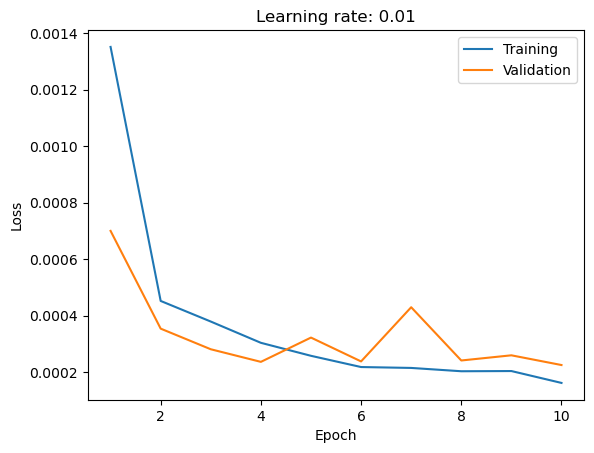
\includegraphics[width=\linewidth]{../plots/localization/learning.png}
        \caption{Learning curve of model with resnet backbone for predicting bounding boxes of heart and lungs}
        \label{fig:organs-localization-learning-curve}
    \end{figure}


    \subsubsection{Result}
    
    After training the model, the model was tested on the provided test set and IoU reported in \cref{tab:organ-localization-result}. We can observe from \cref{tab:organ-localization-result} and \cref{tab:organ-localization-result} that model is able to locate lungs with greater accuracy.

    \begin{table}
        \centering
        \begin{tabular}{cccc}
          \toprule
            & Heart & Lungs & Avg. \\
          \midrule
           IoU & 0.803 & 0.907 & 0.855 \\
          \bottomrule
        \end{tabular}
        \caption{Heart and lungs localization result}
        \label{tab:organ-localization-result}
      \end{table}

 
    \begin{figure*}[htbp]
        \centering
        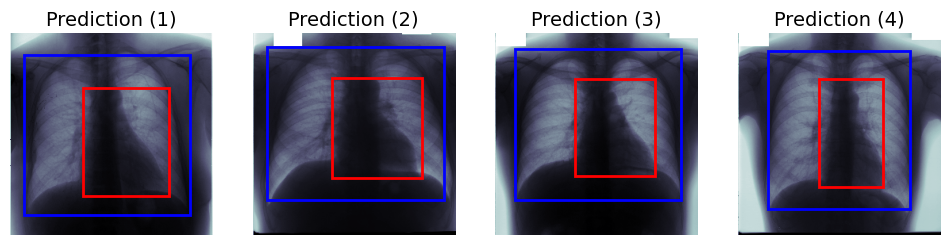
\includegraphics[width=\linewidth]{../plots/localization/result.png}
        \caption{Predicted bounding boxes of heart and lungs}
        \label{fig:organs-localization-result1}
    \end{figure*}